



\begin{description}
\item[Hitting probabilities estimated with direct simulations:] $\approx 0.8180$.  We run 2000 diffusion simulations at each one of the 100 randomly picked initial locations from $\mathcal{B}(0, 1) \setminus (\tilde{A} \cup \tilde{B})$. For each initial location we obtain an estimate of the hitting probability. The mean of these estimates is 0.8180, standard deviation 0.0096. We used time step of size 1e-05. A histogram of the different hitting probabilities, as well as the CHop probability, is shown in Fig. \ref{fig:nontrivial_hitting_prob_test}. The hitting probabilities from different initial locations are in $[0.7980, 0.8450]$, and the $\varepsilon$-flatness condtion holds with $\varepsilon = 0.0470$.

\item[CHop probability]  0.8274, which is in good agreement with the hitting probabilities we obtained from direct simulations. For the region around $x_A$, we used
\begin{equation*}
m = 2, n = 4, 
N_p = 5000, N_b = 10,
N_s = 2000
\end{equation*}
For the region around $x_B$, we used
\begin{equation*}
m = 2, n = 5, 
N_p = 5000, N_b = 10,
N_s = 2000
\end{equation*}
For estimating both of these capacities, we used a 1e-07 time step.
\end{description}

\begin{figure}
	\caption{\label{fig:nontrivial_hitting_prob_test} We picked 100 random locations for $ X_0 \not\in \mathcal{B}(0, 1) \setminus (\tilde{A} \cup \tilde{B})$. For each location we used 2000 simulations to estimate the probability of hitting $A$ before $B$. The histogram of the 100 estimates is shown below. The $\varepsilon$-flatness condtion holds with $\varepsilon = 0.0470,$ and the CHop probability gives good approximation to this narrow range of hitting probabilities.}
	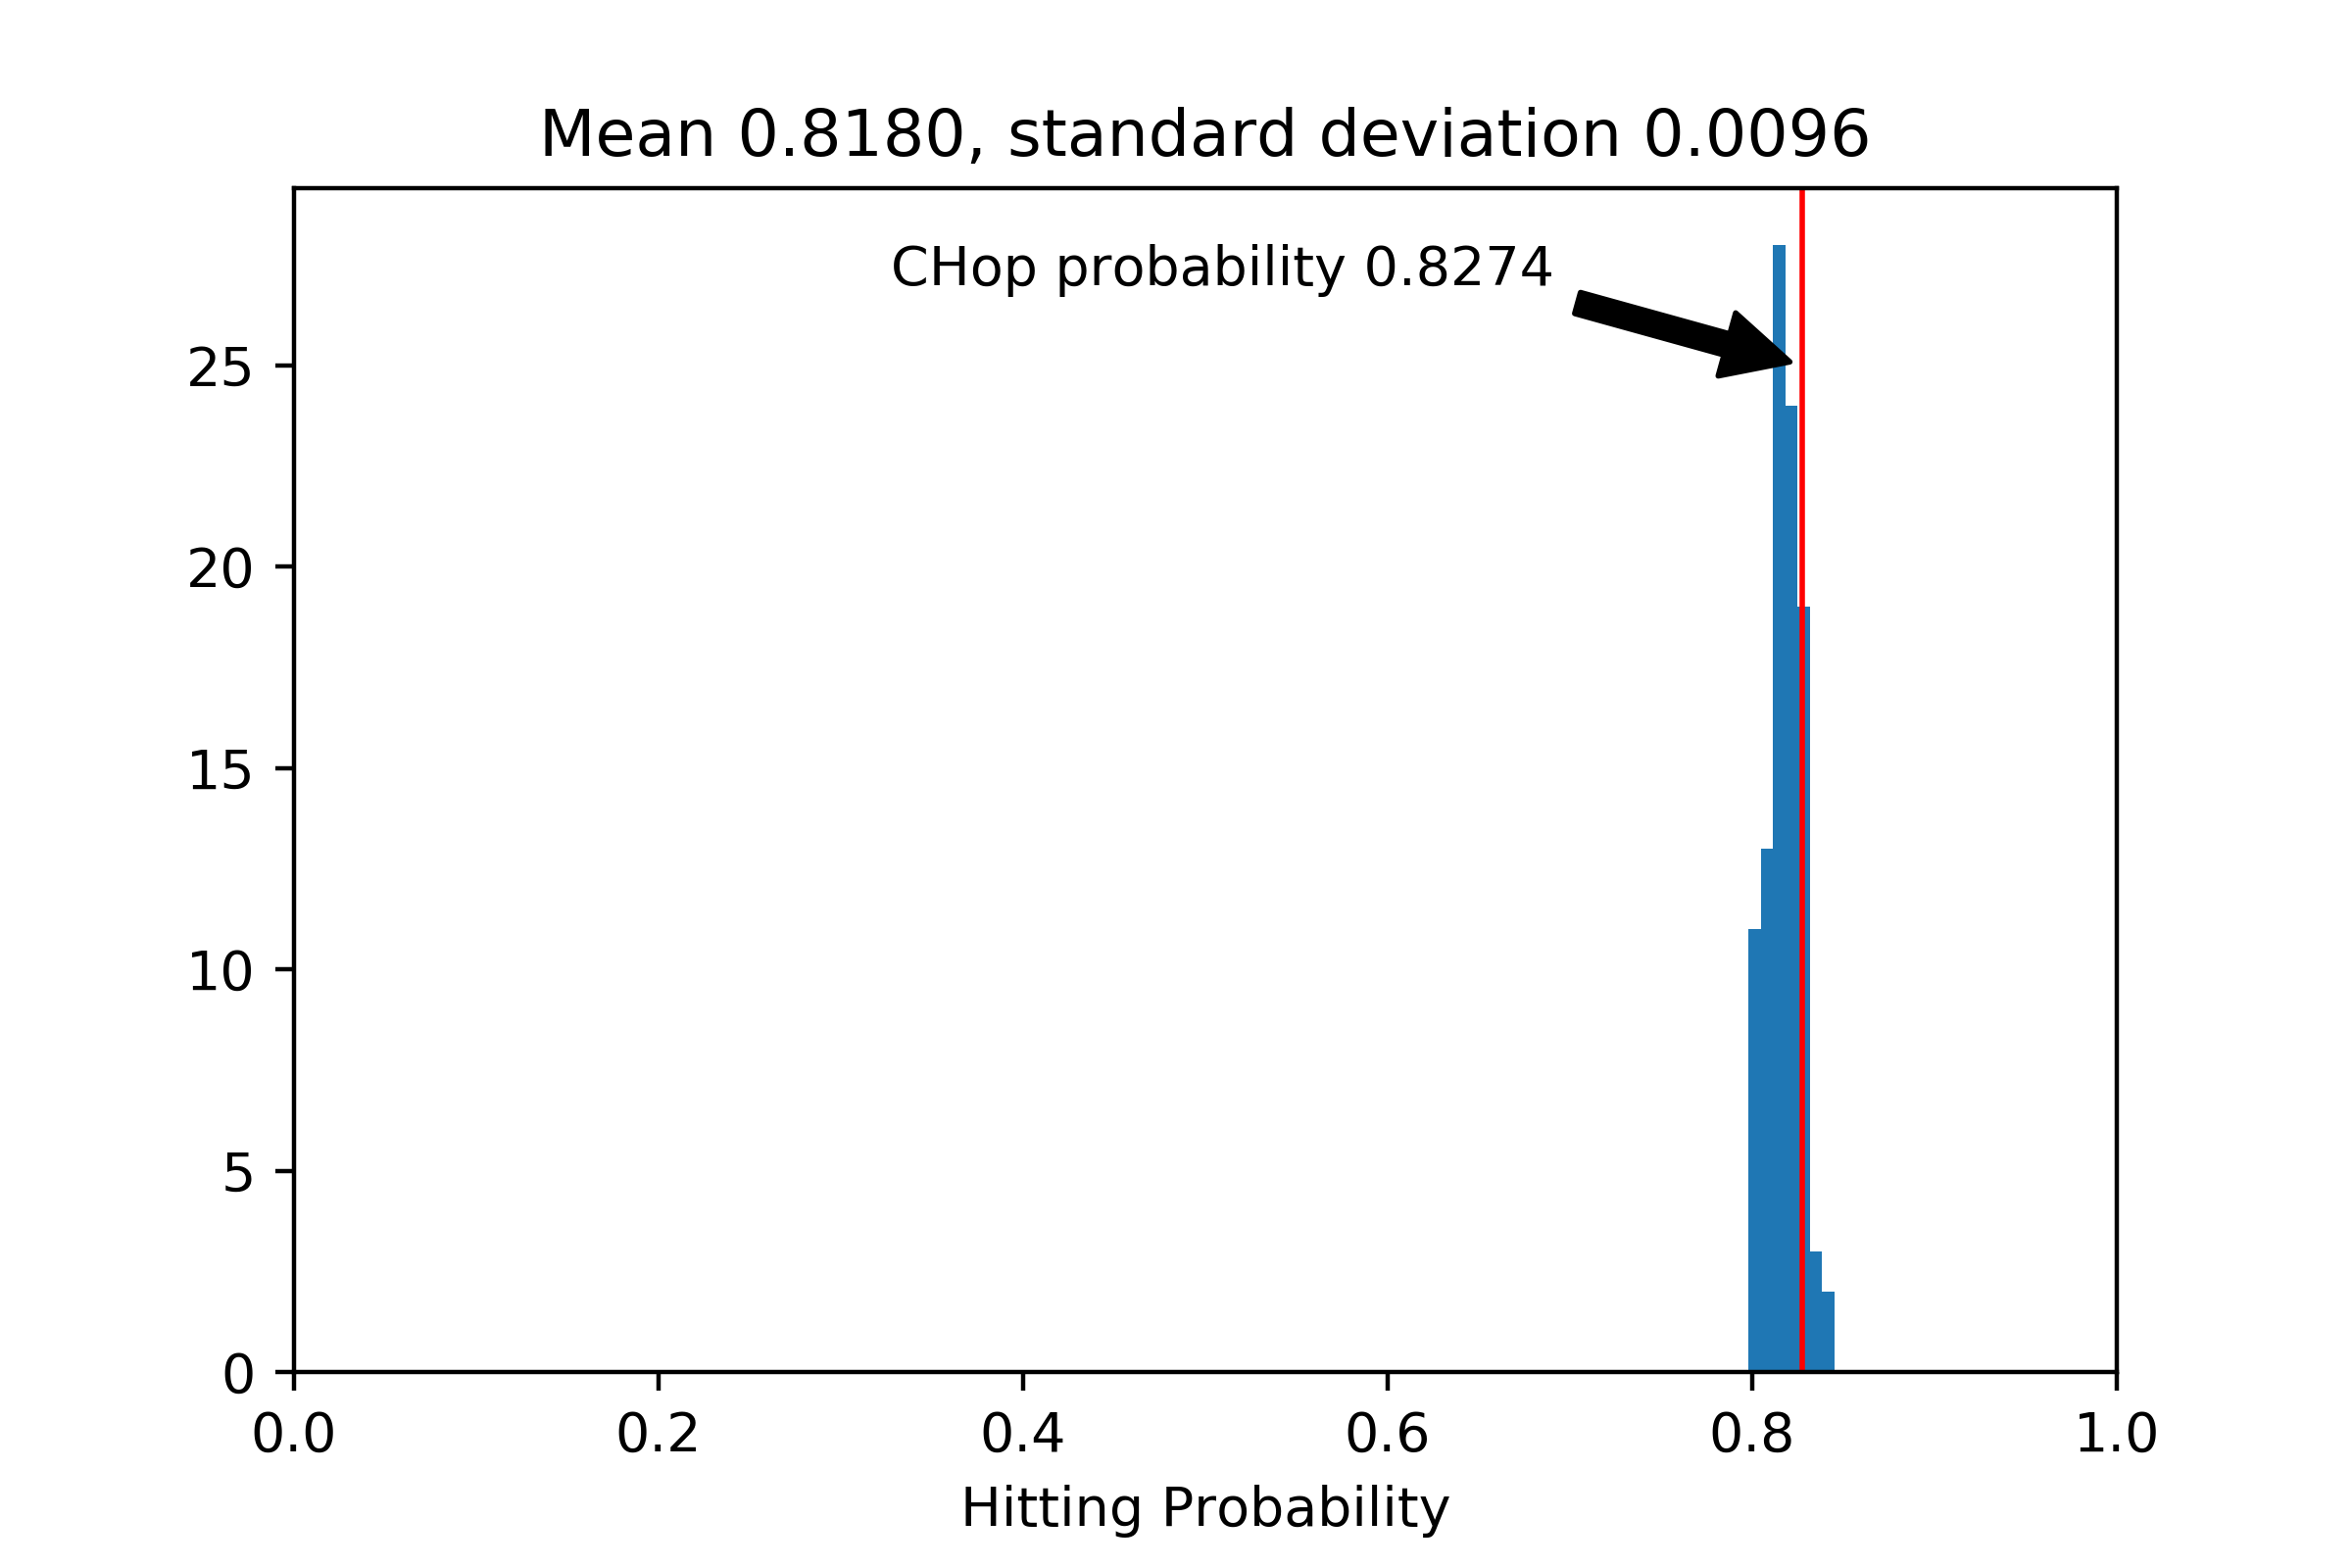
\includegraphics{figs/nontrivial_hitting_prob_hist.png}
\end{figure}
